%        File: pnas1.tex
%     Created: Wed Apr 30 04:00 pm 2014 E
% Last Change: Wed Apr 30 04:00 pm 2014 E
%
\documentclass[letterpaper]{article}
\usepackage[hmargin=0.75cm,vmargin=0.75cm]{geometry}
\usepackage{scrextend}
\usepackage{graphicx}

\usepackage{amsmath}
\usepackage{amssymb}
\usepackage{mathrsfs}
\usepackage{gensymb}
\usepackage{algorithm2e}
\usepackage{amsthm}

\newtheorem*{mydef}{Definition}

\usepackage{framed, color}
\usepackage{soul}
\usepackage[colorlinks=false, urlcolor=blue]{hyperref}
\usepackage{dcolumn}
\usepackage{multirow}
\usepackage{booktabs}
\newcolumntype{d}{D{.}{.}{4.0}}
\newcolumntype{s}{D{.}{.}{1.4}}

\newcommand{\td}[1]{{\color{blu}\hl{TODO: #1}}}

\definecolor{shadecolor}{rgb}{.93,.93,.93}
\definecolor{blu}{rgb}{0,0,1}
\setlength{\parindent}{0cm}
\setlength{\parskip}{4mm plus1mm minus1mm}




\parindent0pt \parskip8pt

\begin{document}
\section*{Supplementary Figures}

\begin{figure}
	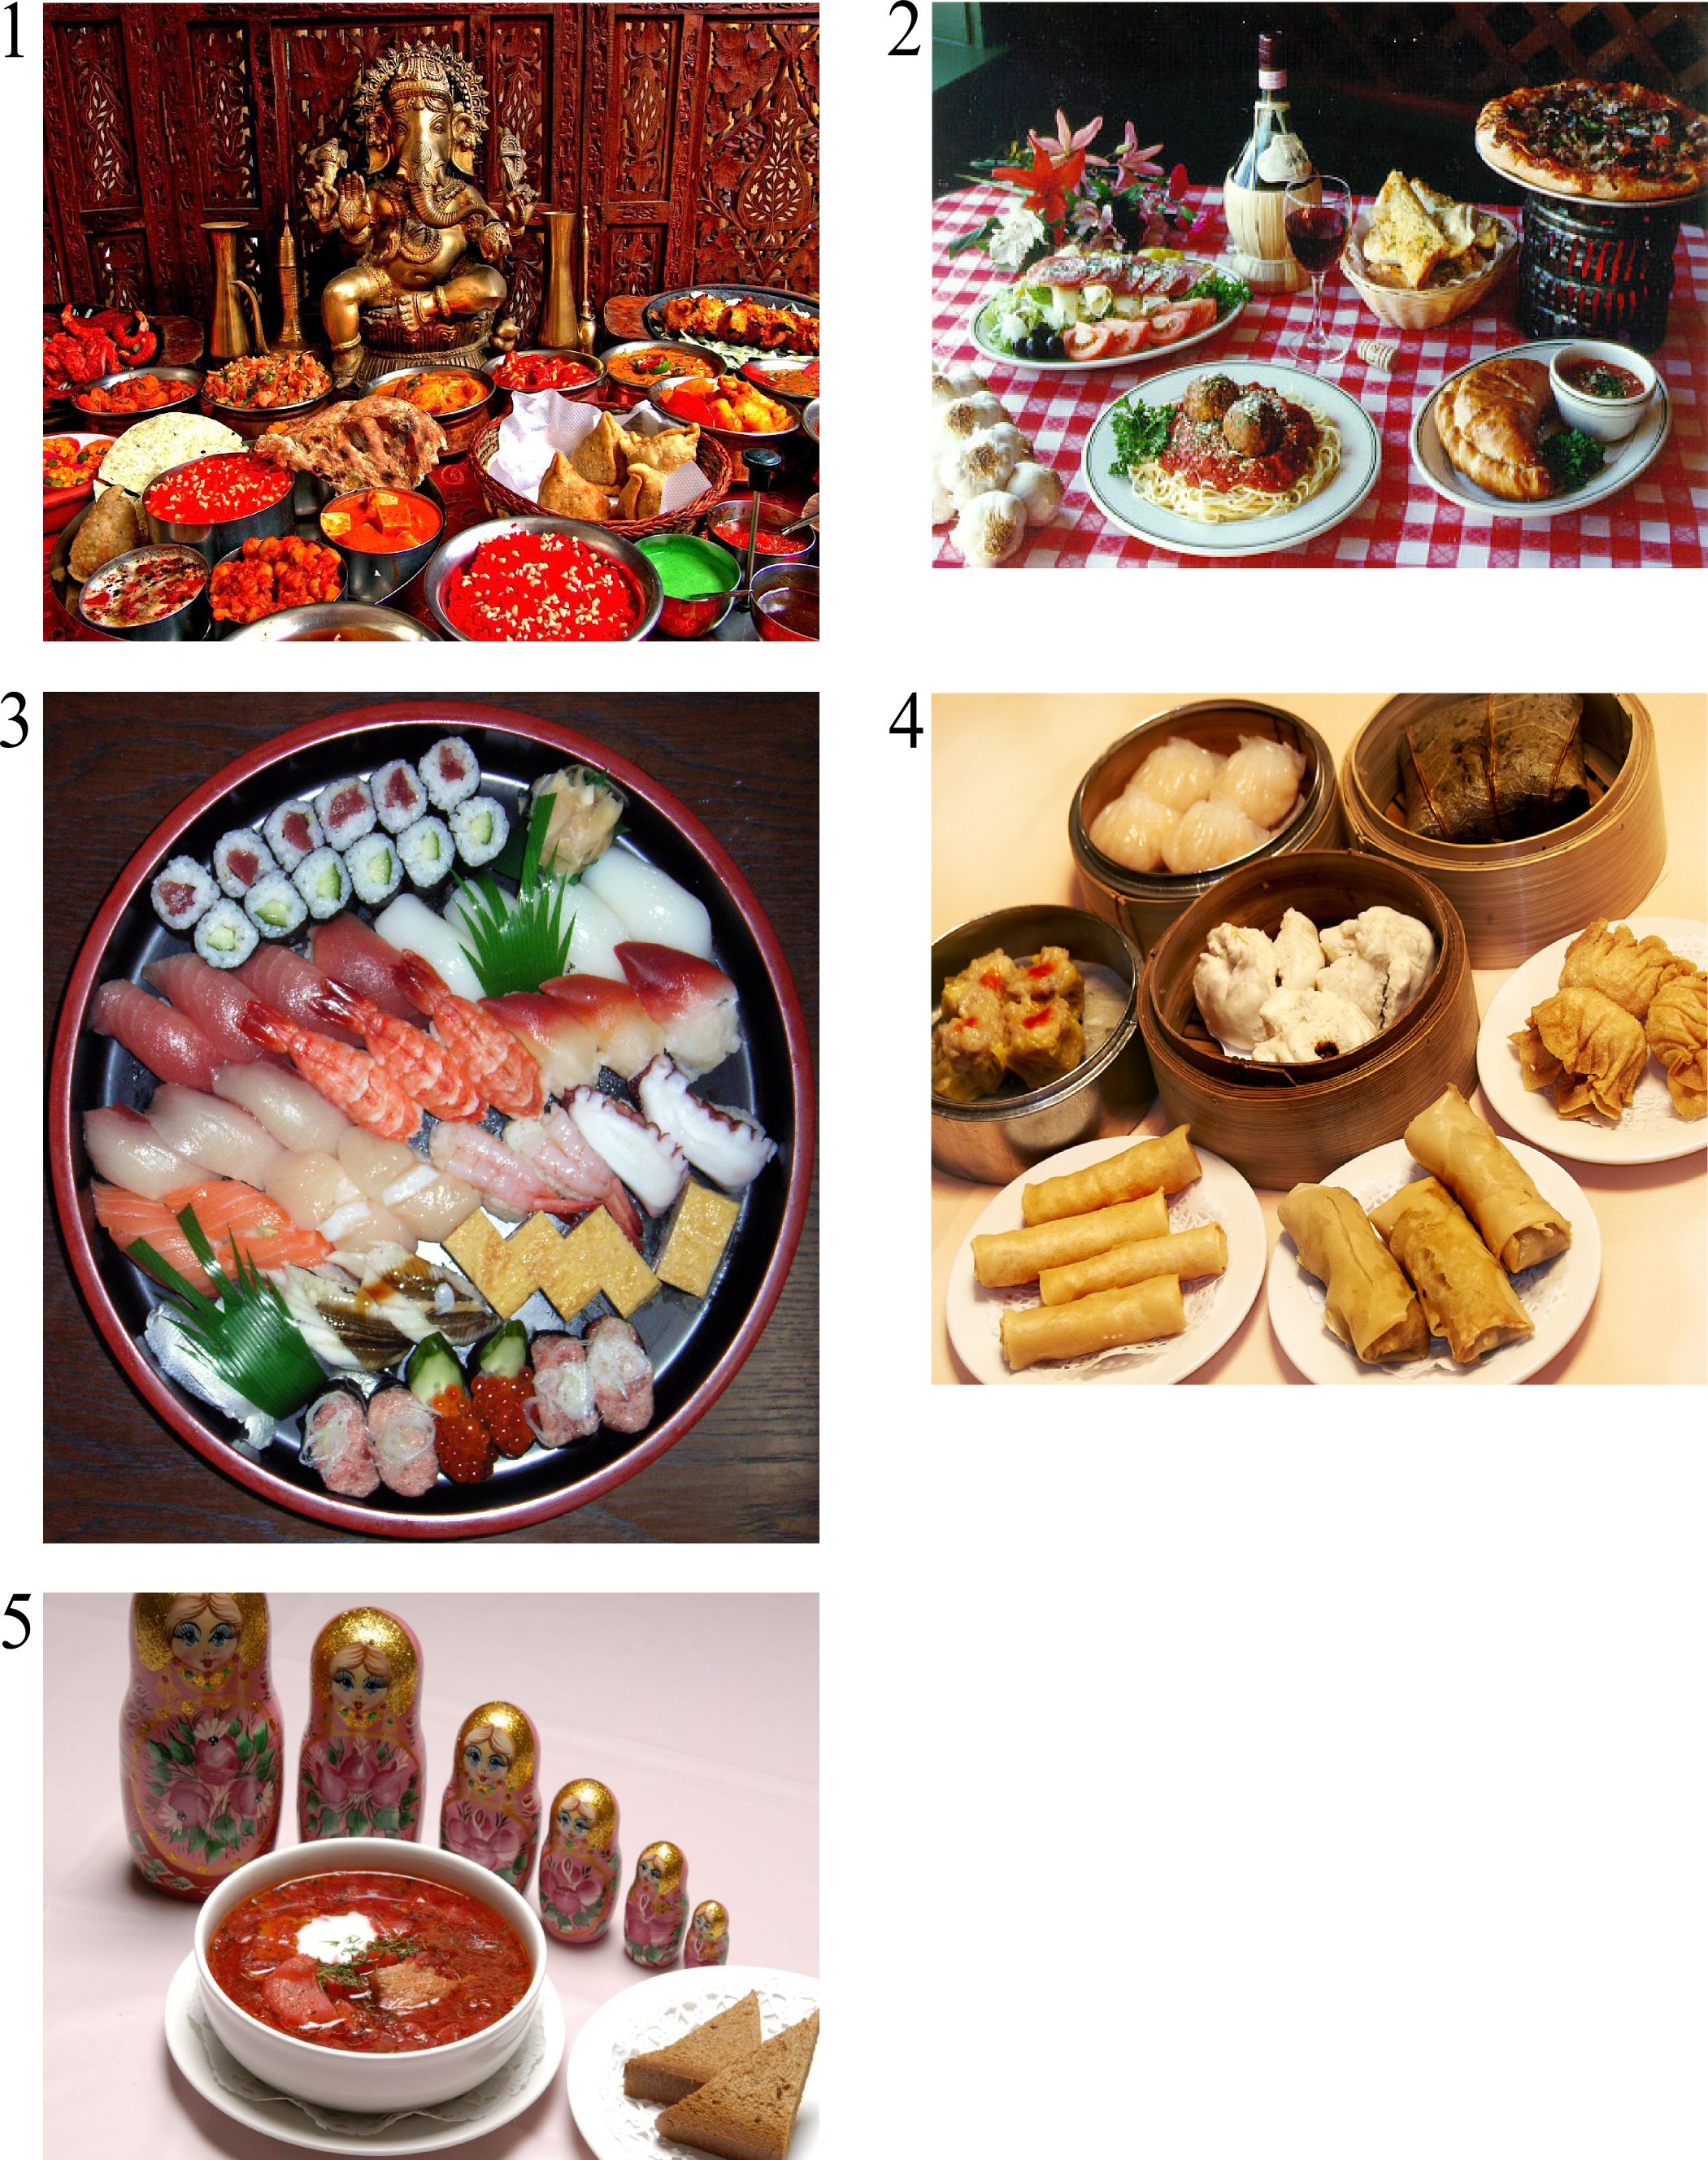
\includegraphics[scale=1.00]{figs/taskImages/testImages.jpg}
	\caption{Testing image set. These images were presented to all workers in 
		the order shown after the priming set of images.}
\end{figure}

\begin{figure}
	\includegraphics[scale=1.00]{figs/taskImages/ambiguous.jpg}
	\caption{ Ambiguous image set. These images were presented to workers from 
		certain treatments (see \textbf{Table 1}) in the order shown.}
\end{figure}

\begin{figure}
	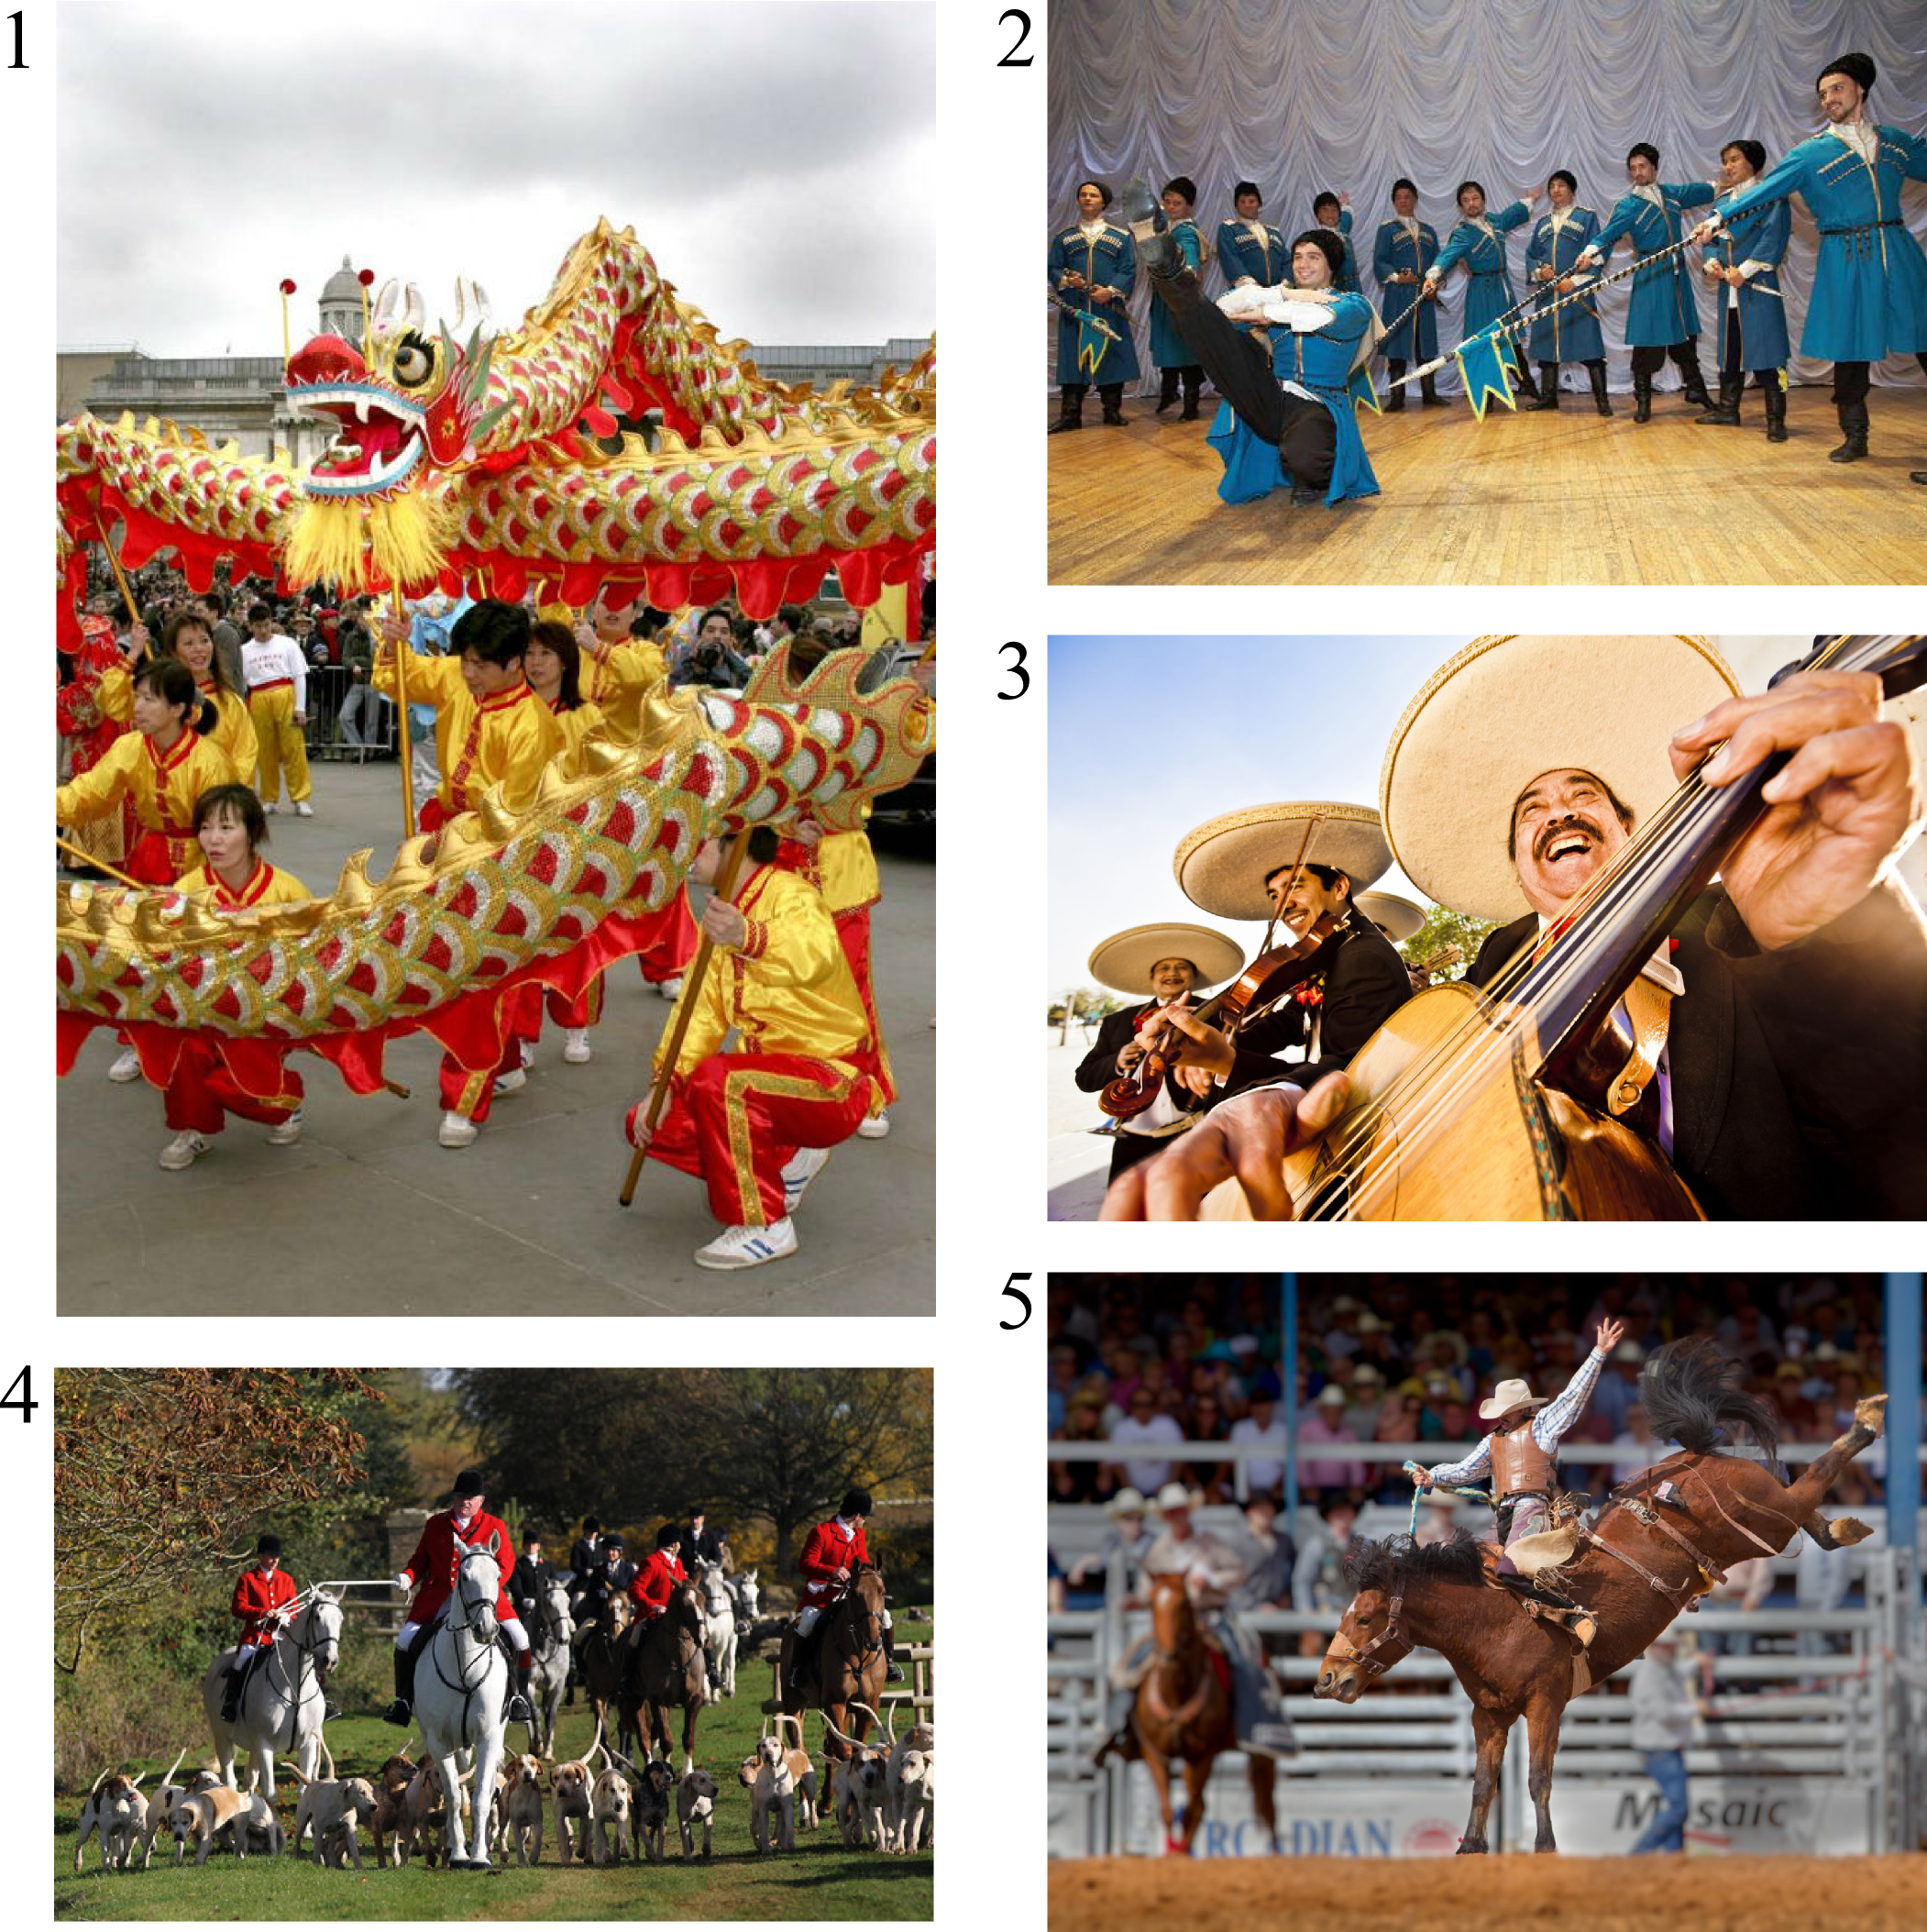
\includegraphics[scale=1.00]{figs/taskImages/cultural.jpg}
	\caption{Cultural image set. These images were presented to workers from 
		certain treatments (see \textbf{Table 1}) in the order shown.}
\end{figure}

\begin{figure}
	\includegraphics[scale=1.00]{figs/taskImages/ingredients.jpg}
	\caption{ Ingredients image set. These images were presented to workers 
		from certain treatments (see \textbf{Table 1}) in the order shown.}
\end{figure}


\end{document}


